% *********************************************************************
% © 2010–2021 Jeremy Sylvestre
%
% Permission is granted to copy, distribute and/or modify this document
% under the terms of the GNU Free Documentation License, Version 1.3 or
% any later version published by the Free Software Foundation; with no
% Invariant Sections, no Front-Cover Texts, and no Back-Cover Texts. A
% copy of the license is included in the appendix entitled “GNU Free
% Documentation License” that appears in the output document of this
% PreTeXt source code. All trademarks™ are the registered® marks of
% their respective owners.
%
% *********************************************************************

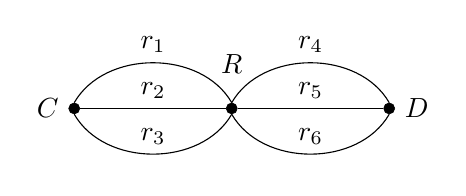
\begin{tikzpicture}[
	vertex/.style={ circle, draw, very thin, fill, inner sep=0pt, minimum size=4pt },
	vertexg/.style={ black!40!white, circle, draw, very thin, fill, inner sep=0pt, minimum size=4pt },
	vertexo/.style={ circle, draw, very thin, inner sep=0pt, minimum size=4pt }
]

\node at (0,0) (C) [vertex,label=left:{$C$}] {};
\node at (2,0) (R) [vertex,label={[yshift=0.25cm]$R$}] {};
\draw (R) to node[above] {$r_2$} (C);
\node at (4,0) (D) [vertex,label=right:{$D$}] {};
\draw (D) to node[above] {$r_5$} (R);
\draw (C.north) to [out=60,in=120] node[above] {$r_1$} (R.north);
\draw (C.south) to [out=-60,in=240] node[above] {$r_3$} (R.south);
\draw (R.north) to [out=60,in=120] node[above] {$r_4$} (D.north);
\draw (R.south) to [out=-60,in=240] node[above] {$r_6$} (D.south);

\end{tikzpicture}
